\chapter{Perspectives}\label{chap:Persp}%\addcontentsline{toc}{chapter}{\nameref{chap:Persp}}
%\markboth{PERSPECTIVES}{}
\mylocaltoc

%Il reste encore beaucoup à faire

%\begin{itemize}
%	\item \'Electroacoustique
%	\begin{itemize}
%		\item Contrôle actif du champ acoustique
%		\item Changement de source principale
%	\end{itemize}
%	\item CFD
%	\begin{itemize}
%		\item Sunfluid
%	\end{itemize}
%	\item Expérimental
%	\begin{itemize}
%		\item Convection naturelle avec charge thermique au CHX
%	\end{itemize}
%\end{itemize}


\section{Expérimentations supplémentaires}

\subsection{\'Etude de la conduction par les parois du noyau thermoacoustique}
La conduction par les parois du noyau thermoacoustique est un facteur très important à prendre en compte. En effet, lorsque le réfrigérateur fonctionne et qu'un gradient de température s'établit le long du régénérateur, un flux de chaleur \og retour \fg{} de conduction apparaît dans le sens opposé au flux de chaleur thermoacoustique. Cependant, contrairement au matériau poreux qui compose le régénérateur, il n'est pas nécessaire que les parois soit conductrice de chaleur. Dans cette section, la \echaf{canette/carter/boîte/enceinte} qui contient les disques de tissu métallique et qui est initialement usinée dans un cylindre d'acier inoxydable est remplacée par une pièce similaire imprimée en plastique. L'ABS est choisi pour la fabrication de ce nouveau contenant plutôt que le PLA, car ce dernier peut se ramollir sous l'action des températures atteintes dans certaines expériences, c'est-à-dire autour de \num{50} à \qty{60}{\degreeCelsius}. Dans le cas de l'ABS, cette température limite d'utilisation est élevée à \qty{100}{\degreeCelsius}.



\section{\'Electroacoustique}

Dans l'optique de poursuivre l'amélioration de cette pompe à chaleur thermoacoustique, l'aspect des sources acoustiques reste à considérer.

\subsection{Contrôle actif}
Le champ acoustique doit être contrôlé avec précision, en particulier l'impédance acoustique et son déphasage au sein du matériau poreux. Dans l'état actuel de la machine, les sources acoustiques sont contrôlées manuellement, et le déphasage inter-sources acoustiques est réglé sur le générateur de signaux. Une étude de l'asservissement de la source secondaire au moyen d'un dispositif de traitement du signal en temps réel tel que le \textit{digital signal processor} ADAU1701 de SigmaDSP (figure~\ref{fig:ActiveControl_ADAU1701}) ou un Teensy~4.1 (figure~\ref{fig:ActiveControl_Teensy41}) est proposée pour la suite de cette thèse, pour atteindre le champ acoustique optimal.



\begin{figure}[!ht]
    \centering
	\begin{subfigure}{.47\textwidth}
		\centering
		\external{fig_ActiveControl_ADAU1701}
		\tikz{\draw(0,0) node{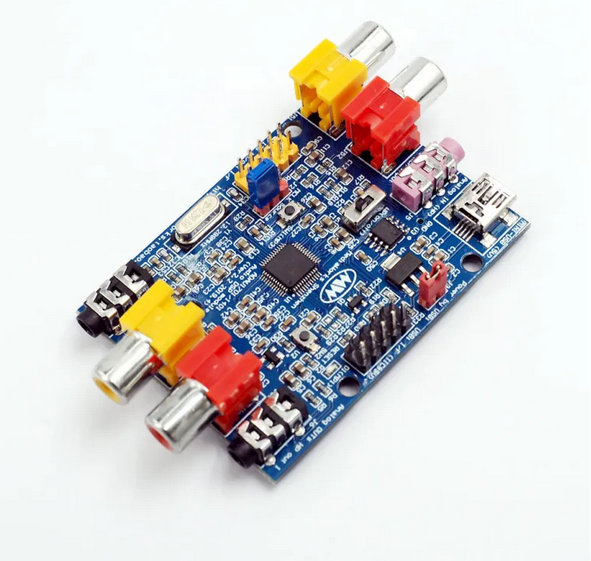
\includegraphics[height=5cm]{../fig/fig_ActiveControl/ADAU1701}};}
		\caption{}
		\label{fig:ActiveControl_ADAU1701}
	\end{subfigure}		
	\begin{subfigure}{.47\textwidth}
		\centering
		\external{fig_ActiveControl_Teensy41}
		\tikz{\draw(0,0) node{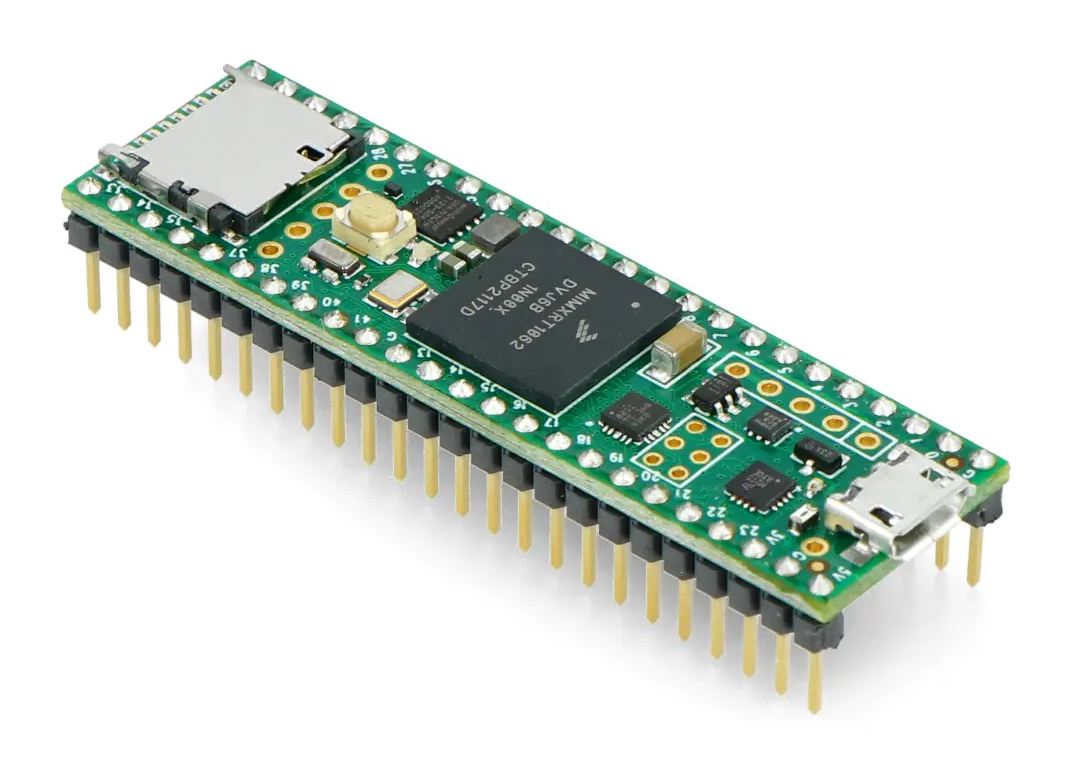
\includegraphics[height=5cm]{../fig/fig_ActiveControl/Teensy41}};}
		\caption{}
		\label{fig:ActiveControl_Teensy41}
	\end{subfigure}	    
    \caption{Dispositif de traitement du signal numérique en temps réel. \subref{fig:ActiveControl_ADAU1701} SigmaDSP ADAU1701 et \subref{fig:ActiveControl_Teensy41} Teensy 4.1}
    \label{fig:ActiveControl}
\end{figure}

Ces cartes sont toutefois sources de retards : les différents calculs réalisés par le processeur, les filtres, les conversions analogique-numérique et numérique-analogique prennent du temps, mais il est possible d'atteindre des retards faibles de l'ordre de \qty{80}{\micro\second}, ce qui correspond à un déphasage de \ang{1.35} à la fréquence de fonctionnement du \textsc{Tacot}, \qty{47}{\hertz}. Cette faible valeur rend possible leur utilisation pour un contrôle du champ acoustique dans la cavité thermoacoustique.

\subsection{Remplacement des sources acoustiques}
\subsubsection{Source principale}
La source acoustique principale est un moteur linéaire. Ce type de source est à la fois onéreux et difficile à se procurer, c'est pourquoi il peut être intéressant d'étudier l'impact sur les performances d'une source alternative. En l'occurrence un haut-parleur du commerce Ciare CSW7012EVO. 

\subsubsection{Source secondaire}



